\pagebreak
\section{teaching}

Inmaculada Garcia Fernandez
\subsection {Joint degrees}

\begin{figure}[h]
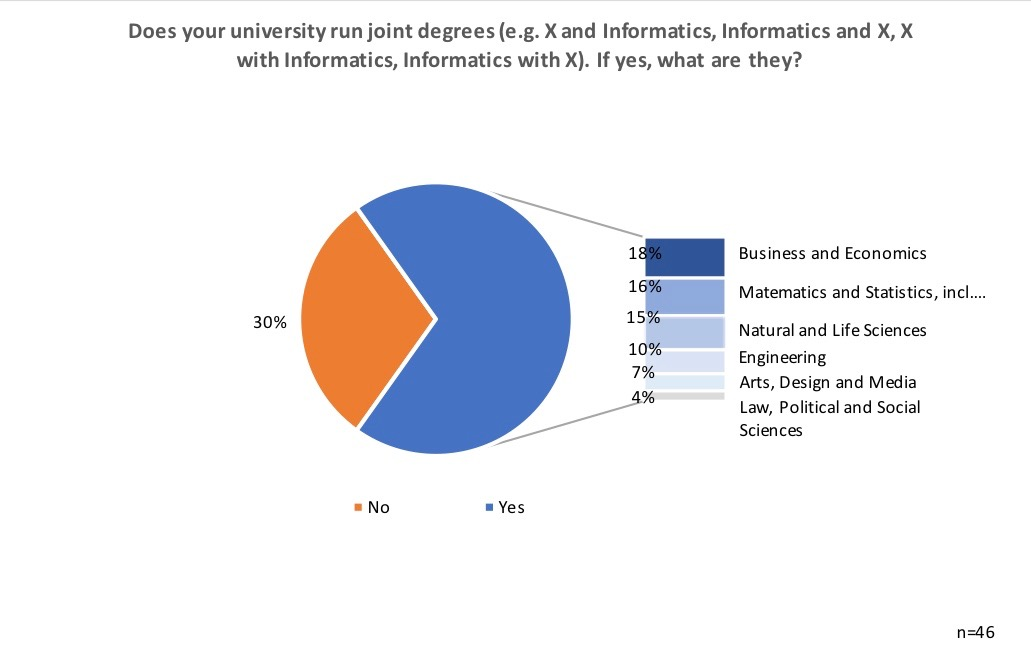
\includegraphics[width = \linewidth]{charts/2a.jpg}
\caption{Does your university run joint degrees?}
\label{sect3:joint}
\end{figure}

30\% of the universities do not run a joint degree that includes Informatics (see Figure~\ref{sect3:joint}. Within this group of universities, some specified that all their programs entail technical aspects of IT, such as programming or data base technology.  At some of these universities there are plans for some joint programmes, e.g. a Data Science BSc programme that joins CS, Maths and Industrial Engineering, and an MSc in Game Design and Production jointly with the Arts School, but these are collaborative initiatives in new directions, where the CS Department is one of the partners or the Business School has their own small Informatics programme for the new degree.

The remaining 70\% of the universities run joint degrees, the most popular joint degrees including Informatics are  Business and Economics (Business Informatics; CS and Business; Computing and Economics; Information systems combining Informatics and Business Administration; CS and Management; Informatics and Economics; Informatics and Finance; Economics and Business Informatics; Data Science and Entrepreneurship) followed by Mathematics and Statistics (Informatics and Mathematics; Data Science; Informatics and Applied Mathematics; Informatics and Statistics), Natural and Life Sciences (Bioinformatics; Informatics and Natural Sciences; CS and Physics; AI for Biomedicine; Precision Medicine; Geoinformatics; Chemistry and Informatics; Biology and Informatics; Informatics Health) and Engineering (Computational Engineering; Computer Engineering; Electronics and Information Engineering; Informatics and Electronics; Informatics and Telecommunications; Informatics and Cybernetics; Informatics and Mechatronics; Informatics and Aerospace Engineering; Informatics and Civil Engineering; Informatics and Industrial Engineering). Joint degrees in informatics plus Arts, Design and Media (Technical Communication; Design Informatics; CS and communication, CS and design; ICT and media; Informatics and information science; Informatics and library science) or Law, Political and Social Sciences (Law and Informatics; Social sciences and Informatics; Data mining for political sciences; Informatics and Psychology; Data science and society; Cognitive Science and AI) are not very frequent at the consulted universities, they represent only the 11\% of the cases. Table \ref{sect3:titles} summarizes  the joint degrees (BSc. and MSc) offered by one or more universities and the countries where they are located.

\begin{table}
\begin{center}
\label{tab:unis}
\begin{tabular}  {|l|l|l|}
\hline
{\bf Level}&{\bf Joint title} & {\bf Countries}\\
\hline
BSc & Economy and Computer Science & Spain, Switzerland \\
\hline
BSc & Economics and Business Informatics & Italy, Switzerland \\
\hline
BSc & Business informatics  &  Austria, Czech, Germany \\
                                             &&Italy, Switzerland, UK, Denmark\\
\hline
BSc & Informatics and Management    & Italy,  UK \\
\hline
BSc & bioinformatics,  & Czech, Denmark, Italy, Switzerland\\
\hline
BSc & Geoinformatics   & Italy\\
\hline
BSc & informatics and Mathematics   & Netherlands, Spain, UK\\
\hline
BSc & Informatics and Statistics   & Spain\\
\hline
BSc & Informatics and Physics   & Spain, UK\\
\hline
BSc & Law and informatics   &  Czech \\
\hline
BSc & Social sciences and informatics   & Czech \\
\hline
BSc & Technical Communication    & Germany, Denmark\\
\hline
BSc & Computational Engineering   & Germany\\
\hline
BSc & Cybernetic  &  Germany\\
\hline
BSc & Mechatronic   & Germany\\
\hline
BSc & INFOTech   & Germany\\
\hline
BSc & Information Science /Library science   & Germany\\
\hline
BSc & Data Science   & Italy, Spain\\
\hline
BSc & ICT and Media   & Italy\\
\hline
BSc & Data Science and Entrepreneurship   & Netherlands\\
\hline
BSc & Data Science and Society   & Netherlands\\
\hline
BSc & Cognitive Science and Art. Intellig.   & Netherlands\\
\hline
BSc & Informatics Health  &Spain\\
\hline
BSc & Informatics and  Engineering   & Spain,  UK\\
\hline
MSc & Data mining with political Sc.  &  Italy\\
\hline
MSc&  Informatics and Psychology   &  Italy\\
\hline
MSc & Comput. Sc. and Engineering & Switzerland\\
\hline
MSc& Bioinformatics  & Switzerland\\
\hline
MSc & Design Informatics    & UK, Denmark\\
\hline
\end{tabular}
\vspace*{.4cm}
\caption{Joint degrees (BSc and MSc) and countries}
\end{center}
\label{ sect3:titles}
\end{table}


\subsection{Plans for changes in joint degrees} 

\begin{figure}[h]
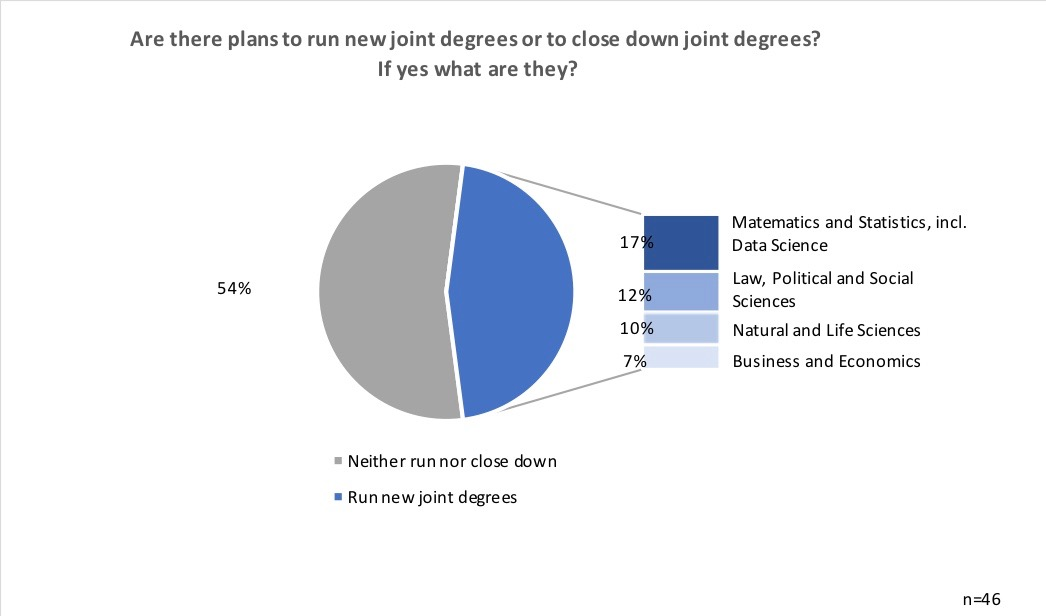
\includegraphics[width = \linewidth]{charts/2b.jpg}
\caption{Are there plans to run new joint degrees or to close down joint degrees?}
\label{sect3:change}
\end{figure}

In general, the situation is  quite stable for those universities that are currently offering joint degrees (see Figure~\ref{sect3:change}). Most of the universities not already offering joint degrees show a significative interest in running new joint degrees. The most popular joint degrees to be run in the future are in the subject of Mathematics and Statistics for which at least eight universities have shown interest (IT University of Copenhagen, University of Edinburgh, University of Oviedo, Aalborg University, Paderborn University, University of Malaga, University of Southern Denmark, Humboldt-Universit\H at zu Berlin, followed by the subject of 
Natural and Life Sciences (University of Bern, University of Stuttgart, University of Lugano, Humboldt-Universit\H at zu Berlin and 
Law, social and political sciences (RWTH Aachen, E\" otv\"os Lor\'and University, University of Edinburgh, University of Stuttgart, Paderborn University) and finally the area of  Business and Economics (University of Edinburgh, University of Bari Aldo Moro, Tilburg University). 

\subsection{Teachers for external departments}
\begin{figure}[h]
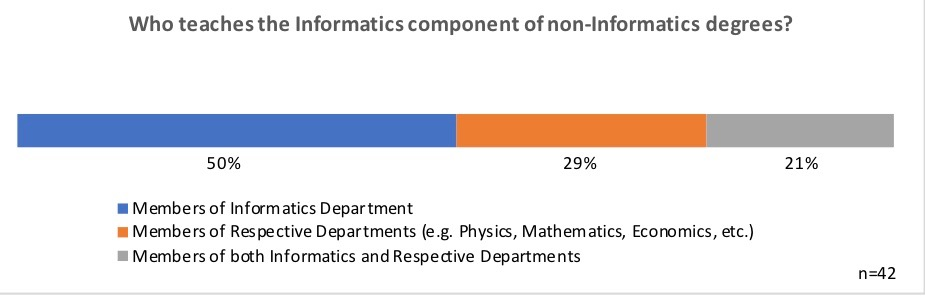
\includegraphics[width = \linewidth]{charts/2c.jpg}
\caption{Who teaches the Informatics component of non-Informatics degrees?}
\label{sect3:teachers}
\end{figure}

The results of the survey indicate that half of the universities (50\%) give the responsibility of teaching informatics subjects to non-informatics degree students to members of the Informatics department (see Figure~\ref{sect3:teachers}). In an additional 21\% of the universities, the responsibility of teaching Informatics is shared among the Informatics department and other departments involved in the joint degree; some of the universities specify that only the general/basic informatics subjects of non-Informatics degrees are taught by academics in the Informatics department (for example programming) but when the subject is related to any particular contents of the degree and the informatics, then the subject is taught by the teachers with profile related with the specific degree. For example, the Bioinformatics of the Biotechnology degree is taught by Chemists. In other universities, informatics component of non-informatics degree programmes is sometimes taught by the informatics department, especially the more advanced levels. Some of the informatics departments have not enough human resources to acquire teaching responsibilities  for non-Informatics degrees . A significative percentage of the universities consulted (29\%) recognize that informatics components of joint degrees are taught by other departments such as Physics, Mathematics, Economics, etc., depending on the subject of the joint degree.

\subsection{Training of Informatics teachers outside of an Informatics department}

\begin{figure}[h]
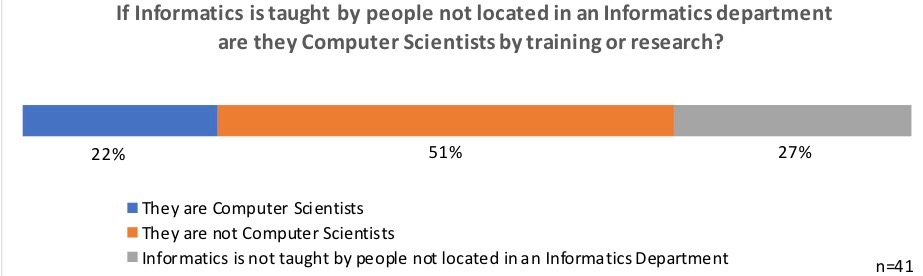
\includegraphics[width = \linewidth]{charts/2d.jpg}
\caption{What training do teachers of Informatics outside of the Informatics department have?}
\label{sect3:whoteaches}
\end{figure}
27\% of the respondents reported that all Informatics taught in their university was taught by members of the Informatics department (see Figure~\ref{sect3:whoteaches}).
Additionally, 22\% of the answers specify that informatics is taught by Computer Scientists. 
Most of the universities participating in the survey recognize that some of the people who teach informatics for students of non-informatics degree do not have a background in Computer Science (51\%). Usually, when the Informatics subjects are  taught by non Computer Scientists, the teachers have a background formation in the same degree the students are following; e.g. electrical engineers in the Electrical Engineering Schools, Economics/Management people at the Business School, Physicists or Engineers in Robotics or Industrial Engineering degrees. Additionally, in some universities the basic informatics courses  are taught by non Computer Scientists.   


\subsection{Final thoughts}

The range of the answers is really broad. For some universities there exists a clear discipline-responsibility (e.g. Paderborn University), but in others there are no clear policy about which department teaches informatics in non-informatics programmes (e.g. RWTH Aachen); lack of human resources prevents the informatics departments from being in charge of teaching informatics subjects in non-informatics degree programmes (e.g. Utrecht University, Università Roma Tre, University of Bari "Aldo Moro",  Tilburg University)
